
% \documentclass[fleqn,10pt]{wlscirep}
% fleqn : left alignment of equation

\documentclass[10pt]{wlscirep}
\usepackage[utf8]{inputenc}
\usepackage{amsmath}
\usepackage{amsbsy}
\usepackage[T1]{fontenc}
\usepackage{soul} % 여러 라인에 걸친 밑줄을 사용하기 위한 패키지

%from here, code for line numbers
\usepackage{lineno}
\linenumbers

\makeatletter
\patchcmd\@maketitle{%
        {%
        \noindent
        \colorbox{color2}{%
            \parbox{\dimexpr\linewidth-2\fboxsep\relax}{%
            \sffamily\small\textbf\\\theabstract
            }%
        }%
        }%
    }{%
        \nolinenumbers{%
        \noindent
        \colorbox{color2}{%
            \parbox{\dimexpr\linewidth-2\fboxsep\relax}{%
            \internallinenumbers \sffamily\small\theabstract
            }%
        }%
        }%
    }
    {\wlog{true}}{\wlog{false}}
    
\makeatother
%end of code for line numbers

\title{Radionuclide Identification for Plastic Scintillation Detectors by Backward Cumulative Channel Sum}
% \linenumbers
\author[1,*]{Myungkook Moon}
\author[1, +]{Ji-Yong So}
\author[2, +]{Byoungil Jeon}
\affil[1]{Korea Atomic Energy Research Institute, Neutron Science Division, Daejeon, 34057, Korea}
\affil[2]{Korea Atomic Energy Research Institute, Applied Artificial Intelligence Section, Daejeon, 34057, Korea}

\affil[*]{moonmk@kaeri.re.kr}

\affil[+]{These authors equally contributed to this work}

\keywords{radiation portal monitor, radionuclide identification}

\begin{abstract}
Accurate identification of radionuclide using plastic scintillation detectors is crucial for screening applications, particularly in radiation portal monitors (RPMs). We present a backward cumulative channel sum (BCCS) method for analyzing gamma-ray spectra acquired with plastic scintillation detectors. The BCCS method transforms pulse-height spectra into cumulative distributions to reduce statistical fluctuations and enhance spectral contrast. This is especially effective under high background and low net count conditions where signals marginally exceed background levels. The method was validated with spectra for single and mixed radionuclides in screening scenarios, showing appropriate performance in isolating radionuclides. The BCCS provides interpretable results with light computational loads, making it suitable for embedded or mobile scanning systems. It can also be directly applied to existing RPMs without additional equipment.  
\end{abstract} 

\begin{document}

\flushbottom
\maketitle
% * <john.hammersley@gmail.com> 2015-02-09T12:07:31.197Z:
%
%  Click the title above to edit the author information and abstract
%
\thispagestyle{empty}

% \noindent Please note: Abbreviations should be introduced at the first mention in the main text – no abbreviations lists. Suggested structure of main text (not enforced) is provided below.

\section*{Introduction}

Radiation portal monitors (RPMs) deployed at national borders play an important role in preventing the smuggling of nuclear and radioactive materials. These systems must detect weak radiation signals from high background radiation counts, requiring high detection efficiency. \ul{To enhance gamma-ray detection efficiency, two principal approaches are typically considered: employing high atomic number (high-Z) materials to increase the interaction probability, or increasing the detector volume to improve geometric efficiency. In practice, the latter approach is often implemented using plastic scintillators, which are widely utilized in radiation portal monitors (RPMs) due to their affordability and ease of manufacturing into large-scale detectors.}\cite{Sicilliano2005Comparision, Bertrand2014Current}

Plastic scintillators have poor energy resolution and absence of full energy peaks in their spectra. Therefore, conventional spectroscopic analysis cannot be applied to the plastic. Furthermore, most of counts are concentrated in the low-energy channels\cite{Sicilliano2005Comparision}, making it difficult to distinguish radionuclides signals from background when the signal intensity is slightly higher than background. 

Recent studies have addressed this challenge using spectral data processing methods, including the energy window methods \cite{Ely2006EWindow, Hevener2013EWindow}, which defines regions-of-interest for each radionuclide, the energy-weighted method \cite{Lee2020EWeight}, which emphasizes spectral shape near Compton Edges. There are several template matching techniques, e.g., spectral angular mapping \cite{Paff2017Spectral} and inverse calibration matrix \cite{Kim2019InvMat}, which compare measured data with pre-defined radionuclide dataset. In parallel, Kim et al. demonstrated the feasibility of artificial neural network-based radionuclide identification\cite{Kim2019ANN}, and another group applied energy-weighted preprocessing combined with convolutional neural networks to improve radionuclide identification performance in RPM applications\cite{Lee2023Radionuclide}. 

Building on these advances, our previous work introduced artificial intelligence (AI)-driven methods for plastic scintillation detectors. These include a machine learning approach \cite{Jeon2021CompML}, a multitask deep learning model for pseudo-gamma spectroscopy\cite{Jeon2021PseudoGamma}, and a deep learning model with its explanation\cite{Jeon2023Explanation}. These approaches demonstrated improved nuclide identification, even in the absence of full-energy peaks. 

In practical settings, additional challenges arise. Cargo containers often induce baseline suppression—also known as the shadow effect—where both background and source counts are significantly reduced. Observational studies report count losses exceeding 30\%, depending on vehicle geometry and panel position\cite{LoPresti2006BaselineSuppression}. Such suppression degrades gross-count or peak-based methods and reduces identification confidence, especially in low-count scenarios. 

This paper presents a backward cumulative channel sum (BCCS) to address these limitations. BCCS transforms raw plastic scintillator spectra into \ul{backward} cumulative form, emphasizing global spectral structure while reducing high-frequency uncertainties. Unlike conventional background subtraction or AI-based methods that require extensive training or calibration, BCCS is computationally lightweight, interpretable, and well suited for real-time embedded systems. Its performance was evaluated through experiments with single and multiple radionuclides, and it was verified that the BCCS enables accurate and stable nuclide identification—even under low-count and baseline-suppressed conditions—without relying on peak-based features or machine learning. This work provides a practical, scalable, and calibration-free solution for radionuclide identification in radiation portal monitoring systems using plastic scintillators.

\section*{Methods}

\subsection*{Spectral Preprocessing: Backward Cumulative Channel Sum}

Most radiation portal monitors employ plastic scintillators, which provide high detection efficiency due to their large effective volume but suffer from poor spectroscopic performance. As a result, additional processing techniques are required to identify radionuclides, particularly when source intensity is lower than background radiation, i.e., under low net-count conditions. In such cases, signal processing methods that enhance spectral features and compensate for detector limitations become essential. To address these challenges, we propose the Backward Cumulative Channel Sum (BCCS) method, derived as follows.

Given a raw pulse-height spectrum $\mathbf{C} = [C_1, C_2, \ldots, C_N]$, where $C_i$ denots the count in channel $i$, the corresponnding BCCS spectrum $\mathbf{B} = [B_1, B_2, \ldots , B_N]$ is defined as follows: 

\begin{equation}
B_i = \sum_{j=i}^N C_i.
\end{equation}

In contrast to the conventional cumulative spectrum, which sums counts from the first channel up to channel $i$, the BCCS accumulates counts from channel $i$ to the final channel. As a result, the BCCS spectrum is monotonically decreasing, and the value at each bin represents the total counts from that bin to the end of the spectrum. This operation helps to reduce statistical fluctuations in relatively higher energy channels while preserving the overall spectral shapes, making it particularly useful low net-count measurements in RPM. 

\subsection*{Background Compensation Techniques}

Under weak source conditions with a short measuring period, background radiation is dominant in measured spectra and the spectra have poor counting statistics. In this case, it is necessary to compensate for background contributions in the spectra and to improve signal-to-noise ratio for reliable radionuclide identification. 

In this study, we propose two background compensation strategies: (a) direct subtraction and (b) ratio-based normalization, each providing unique advantages in terms of physical interpretability and statistical robustness.  

\subsubsection*{(a) Direct Subtraction}

Direct subtraction obtains the net spectrum by subtracting the background BCCS spectrum from that of the source. Let $\mathbf{B}^X$ and $\mathbf{B}^\textrm{bkg}$ denote the BCCS spectra of source $X$ and background, respectively. The net spectrum $\mathbf{S}^X$ is then given by

\begin{equation}
\mathbf{S}^X =  \mathbf{B}^X - \mathbf{B}^{\textrm{bkg}}
\end{equation}

This operation yields an interpretable estimate of the source contribution while preserving the count scale. Owing to the cumulative nature of BCCS, negative values rarely occur even for weak signals, making the method inherently robust against over-subtraction.

\subsubsection*{(b) Ratio-Based Normalization} 

Ratio-based normalization emphasizes relative spectral deviations by dividing the source BCCS spectrum by the background spectrum. For source $\mathbf{R}^X$, the normalized spectrum $\mathbf{R}^X=[R^X_1,\ldots,\,R^X_N]$ is defineds as

\begin{equation}
R^X_i = \left(\dfrac{B^X_i}{B^{\textrm{bkg}}_i}\right) -1.
\end{equation}

This produces a dimensionless representation that highlights local contrasts while suppressing global count variability, making it particularly effective when source signals are only slightly above background levels.


Direct subtraction provides an absolute estimate of source contributions, while ratio-based normalization highlights relative deviations from background. By combining these complementary perspectives, both methods ensure flexibility and robustness under diverse measurement conditions.

\subsection*{Radionuclide Activity Estimation via Linear Spectral Unfolding}


For quantitative analysis, the net or ratio-normalized spectrum can be modeled as a linear combination of reference spectra:

\begin{equation}
\textbf{S}^{\textrm{tot}} \approx \sum_{X} \alpha_X \textbf{S}^{X}
\end{equation}

\noindent where $\alpha_X$ denotes the contribution of radionuclide $X$. The coefficients $\alpha_X$ are determined by solving the non-negative least squares (NNLS) problem

\begin{equation}
\min_{\alpha_X \ge 0} \left\| \textbf{S}^{\textrm{tot}} - \sum_{X} \alpha_X \textbf{S}^{X}\right\|^2 .
\end{equation}

This approach yields physically meaningful, non-negative activity estimates, even under spectral overlap or low-count conditions. Applied to both BCCS and ratio-normalized spectra, it enables reliable decomposition of mixed radionuclide measurements.

\section*{Results}

%Up to three levels of \textbf{subheading} are permitted. Subheadings should not be numbered.

\subsection*{Spectral Transformation}

Raw spectra in Figure \ref{fig:bkgref} were acquired for background radiation and three reference sources (Am-241, Cs-137, and Co-60) using a large-volume plastic scintillation detector (30 cm × 180 cm × 5 cm). \ul{As expected These spectra exhibited broad Compton continua} with poor energy resolution, and most counts were concentrated in the low-channel region (channels < 50), reflecting the known limitations of plastic scintillator detectors.

Application of the BCCS method transformed these raw spectra into smooth, monotonically decreasing cumulative distributions(Figure \ref{fig:channelsum}). This process reduced statistical fluctiations in high-channel region while preserving global spectral structure. The resulting enhancement of spectral contrast improved the separability of source and background spectra, particularly under low-count conditions.

\subsection*{Background Compensation and Source Separation}

Two background compensation methods—direct subtraction and ratio-based normalization—were applied to the BCCS spectra. Direct subtraction effectively isolated net source signals by removing background contributions, producing interpretable spectra that retained source-specific decay patterns (Figure \ref{fig:csn}). This approach also remained valid for mixed-source measurements, where the resulting spectra preserved mixture-dependent features reflecting the relative contributions of each radionuclide (Figure \ref{fig:csbrs}).
Ratio-based normalization (Figures \ref{fig:csbs} and \ref{fig:fi_CSBRS}) emphasized proportional deviations from background, revealing characteristic patterns even under low-count conditions. By suppressing global count variability, this method enhanced pattern recognition and maintained robustness when source signals only slightly exceeded background levels.

\subsection*{Quantitative Analysis via Spectral unfolding}

The distinct spectral patterns obtained through background subtraction and ratio normalization provided a stable basis for linear spectral unfolding. By solving NNLS problems, the mixed-source spectra were decomposed into their constituent radionuclide contributions. This quantitative analysis showed that the proposed methods can estimate activities of individual nuclides without relying on energy resolution or the existence of full energy peaks in the spectra, addressing a critical limitation of plastic scintillation detectors.

\subsection*{Demonstration in Food Radiation Screening}

The proposed methods were evaluated in a realistic food radiation screening scenario involving Cs-137 and K-40. Measurements were conducted using a plastic scintillation detector with dimensions of 30 cm × 40 cm × 5 cm (W×D×H) covered by 5-cm-thick lead plates. The measuring period was 10 seconds for each spectrum. A reference source was used for Cs-137, and and 600 g of potassium chloride (KCl) was used as the K-40 source, with an activity of approximately 1000 Bq.

Figure \ref{fig:fi_spe} depicts measured spectra for K-40, Cs-137, and background radiation from a plastic scintillation detector. As shown in the figure, the counts in the measured spectra were approximately 10\% higher than that of background spectrum. It demonstrates that the detector system has sufficient sensitivity to distinguish low-level contamination from background radiation, when appropriate spectral processing methods are utilized. The following figures represent radio-based normalization (Figure \ref{fig:fi_csn}) and direct subtraction (Figure \ref{fig:fi_csbs}) results, verifying that proposed methods clearly separated the spectral features of Cs-137 and K-40. This implies that a large volume plastic scintillation detector has sufficient capability to discriminate anthropogenic contamination from naturally occurring potassium radiation in food products such as seaweed, bananas, or salt. These results validate that the proposed methods as a realistic and robust solution for food safety monitoring, with potential extension to security and environmental radiation screening applications.

\section*{Discussion}

This study investigated spectral data processing methods to improve radionuclide identification performance using plastic scintillation detectors for RPMs or food screening systems. The proposed methods—BCCS, direct subtraction, and ratio-based normalization—were validated through experiments involving both single and mixed radionuclides.

The BCCS method demonstrated its effectiveness in reducing high-frequency statistical uncertainties while enhancing overall spectral contrast, enabling more reliable analysis of low-resolution spectral data. Direct subtraction provided interpretable net spectra by isolating source contributions from background, while ratio-based normalization emphasized relative spectral deviations, improving pattern recognition under low-count or variable background conditions.

Both methods retained distinct spectral features in mixed-source scenarios, supporting quantitative analysis through linear spectral unfolding. The NNLS method enabled the estimation of individual radionuclide contributions without relying on energy peak resolution, one of the limitations of plastic scintillation detectors.

Simulation validation showed good agreement with experimental measurements, with calculated-to-measured ratios ranging from 0.77 to 0.97 across various conditions. This confirmed the reliability of the computational model for system performance prediction and optimization.

Importantly, the practical demonstration using Cs-137 and K-40 in a food radiation screening setup highlighted the system's sensitivity to subtle differences—approximately 10\% above background levels—with less than 5\% relative statistical uncertainty based on repeated measurements. This demonstrates its reliability for detecting weak radioactive contamination in food products.

Beyond food safety, this capability extends to broader applications such as border security, cargo inspection, scrap metal recycling, and environmental radiation monitoring, where differentiating between anthropogenic and naturally occurring radiation is critical.

In summary, the complementary strengths of direct subtraction and ratio-based normalization suggest that a hybrid approach may offer optimal performance across diverse operational scenarios. Future work will focus on integrating these methods into field-deployable RPM systems, validating performance in dynamic environments, and extending the framework to incorporate real-time background modeling and adaptive detection algorithms.

\section*{Conclusion}

This study presented a robust and efficient methodology for radionuclide identification for plastic scintillation detectors in radiation portal monitoring and food safety applications. The proposed methods—Backward Cumulative Spectral Normalization, direct subtraction, and ratio-based normalization—were systematically validated by simulations and experiments. Key findings of this study include:

• Enhanced Spectral Robustness: BCCS effectively suppressed statistical uncertainties while preserving global spectral features.

• Reliable Background Compensation: Direct subtraction and ratio-based normalization enabled accurate separation of source signals from background radiation.

• Quantitative Analysis Capability: Linear spectral unfolding with NNLS provided physically meaningful estimates of mixed radionuclide contributions.

• Model Validation: Simulation results showed good agreement with experimental data, supporting predictive system design.

• Practical Demonstration: The system successfully detected low-level Cs-137 and K-40 contamination in food, with less than 5\% statistical uncertainty, confirming its applicability to real-world scenarios such as food safety monitoring, border control, cargo screening, and scrap metal recycling.

These results confirm that the proposed methods offer a scalable and interpretable radionuclide identification solution for radiation detectors with poor energy resolution. Future research will aim to validate these techniques in various operational scenarios and enhance their integration into next-generation radiation monitors.


% \noindent LaTeX formats citations and references automatically using the bibliography records in your .bib file, which you can edit via the project menu. Use the cite command for an inline citation, e.g.\cite{Hao:gidmaps:2014}.

% For data citations of datasets uploaded to e.g. \emph{figshare}, please use the \verb|howpublished| option in the bib entry to specify the platform and the link, as in the \verb|Hao:gidmaps:2014| example in the sample bibliography file.

\section*{Acknowledgements}

This research was supported by the Ministry of Oceans and Fisheries, Korea, through the Korea Institute of Marine Science \& Technology Promotion (KIMST) under Project No. 20200611. The authors acknowledge the use of ChatGPT (OpenAI) for language refinement and editorial assistance during the preparation of this manuscript. All scientific content, interpretations, and conclusions presented herein were solely developed and validated by the authors.

\section*{Author contributions statement}
M. Moon conceived the study and performed the experiments. J. So developed the analysis software and performed signal processing. B. Jeon synthesized the test datasets and supported evaluation. All authors contributed to writing and reviewing the manuscript.

\bibliography{./biblio}

\section*{Additional information}

% To include, in this order: \textbf{Accession codes} (where applicable); \textbf{Competing interests} (mandatory statement). 

% The corresponding author is responsible for submitting a \href{http://www.nature.com/srep/policies/index.html#competing}{competing interests statement} on behalf of all authors of the paper. This statement must be included in the submitted article file.


\begin{figure}[ht]
\centering
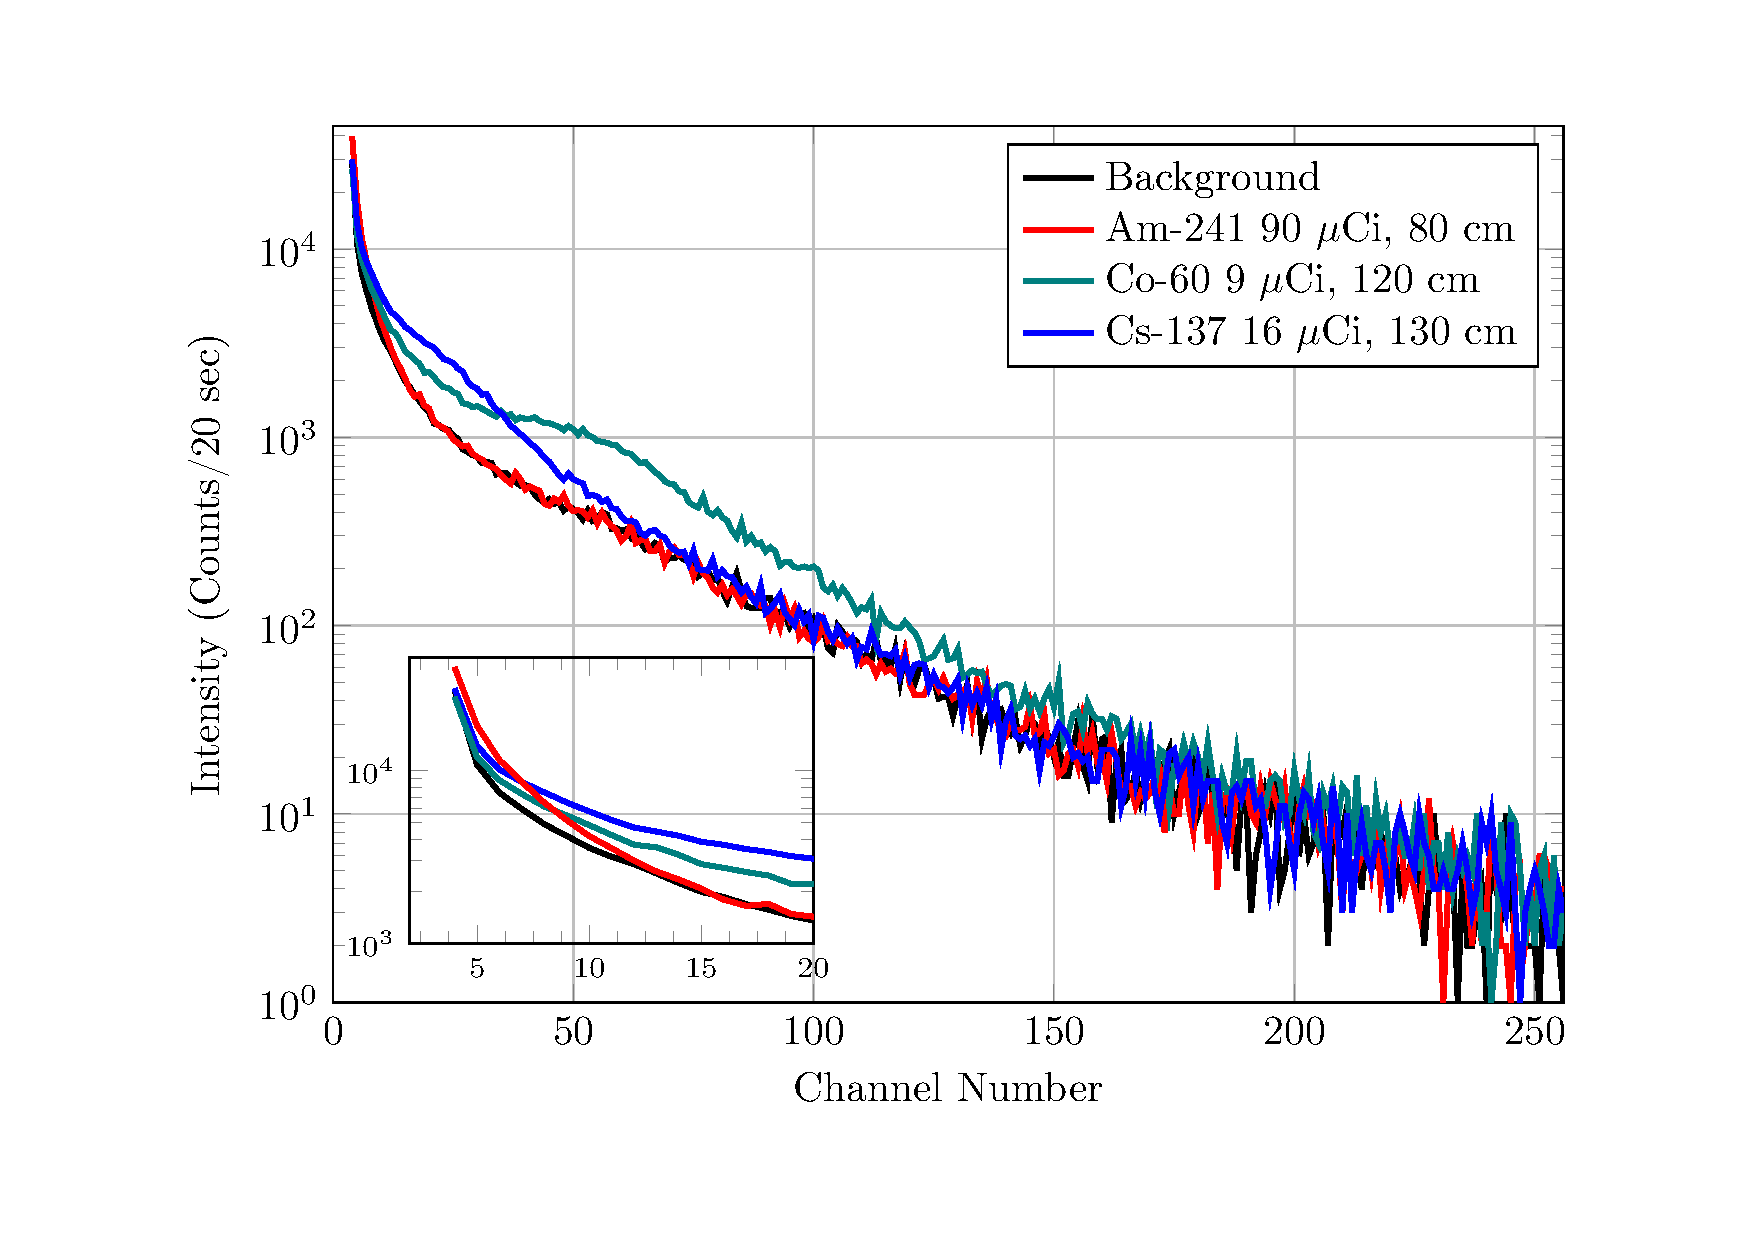
\includegraphics[width=\linewidth]{figure/fig01_bkgref.pdf}
\caption{Raw gamma-ray spectra acquired from background (black) and reference radionuclides, including Am-241 (red), Co-60 (green), and Cs-137 (blue). The spectra were measured under typical radiation portal monitoring conditions. All spectra exhibit broad, featureless distributions dominated by Compton scattering, with most counts concentrated in the low-energy region (channels $\le$ 60). \ul{The inset shows that the difference between the background and Am-241 spectra is marginal and seen only in the low-channel region.}}
\label{fig:bkgref}
\end{figure}

\begin{figure}[ht]
\centering
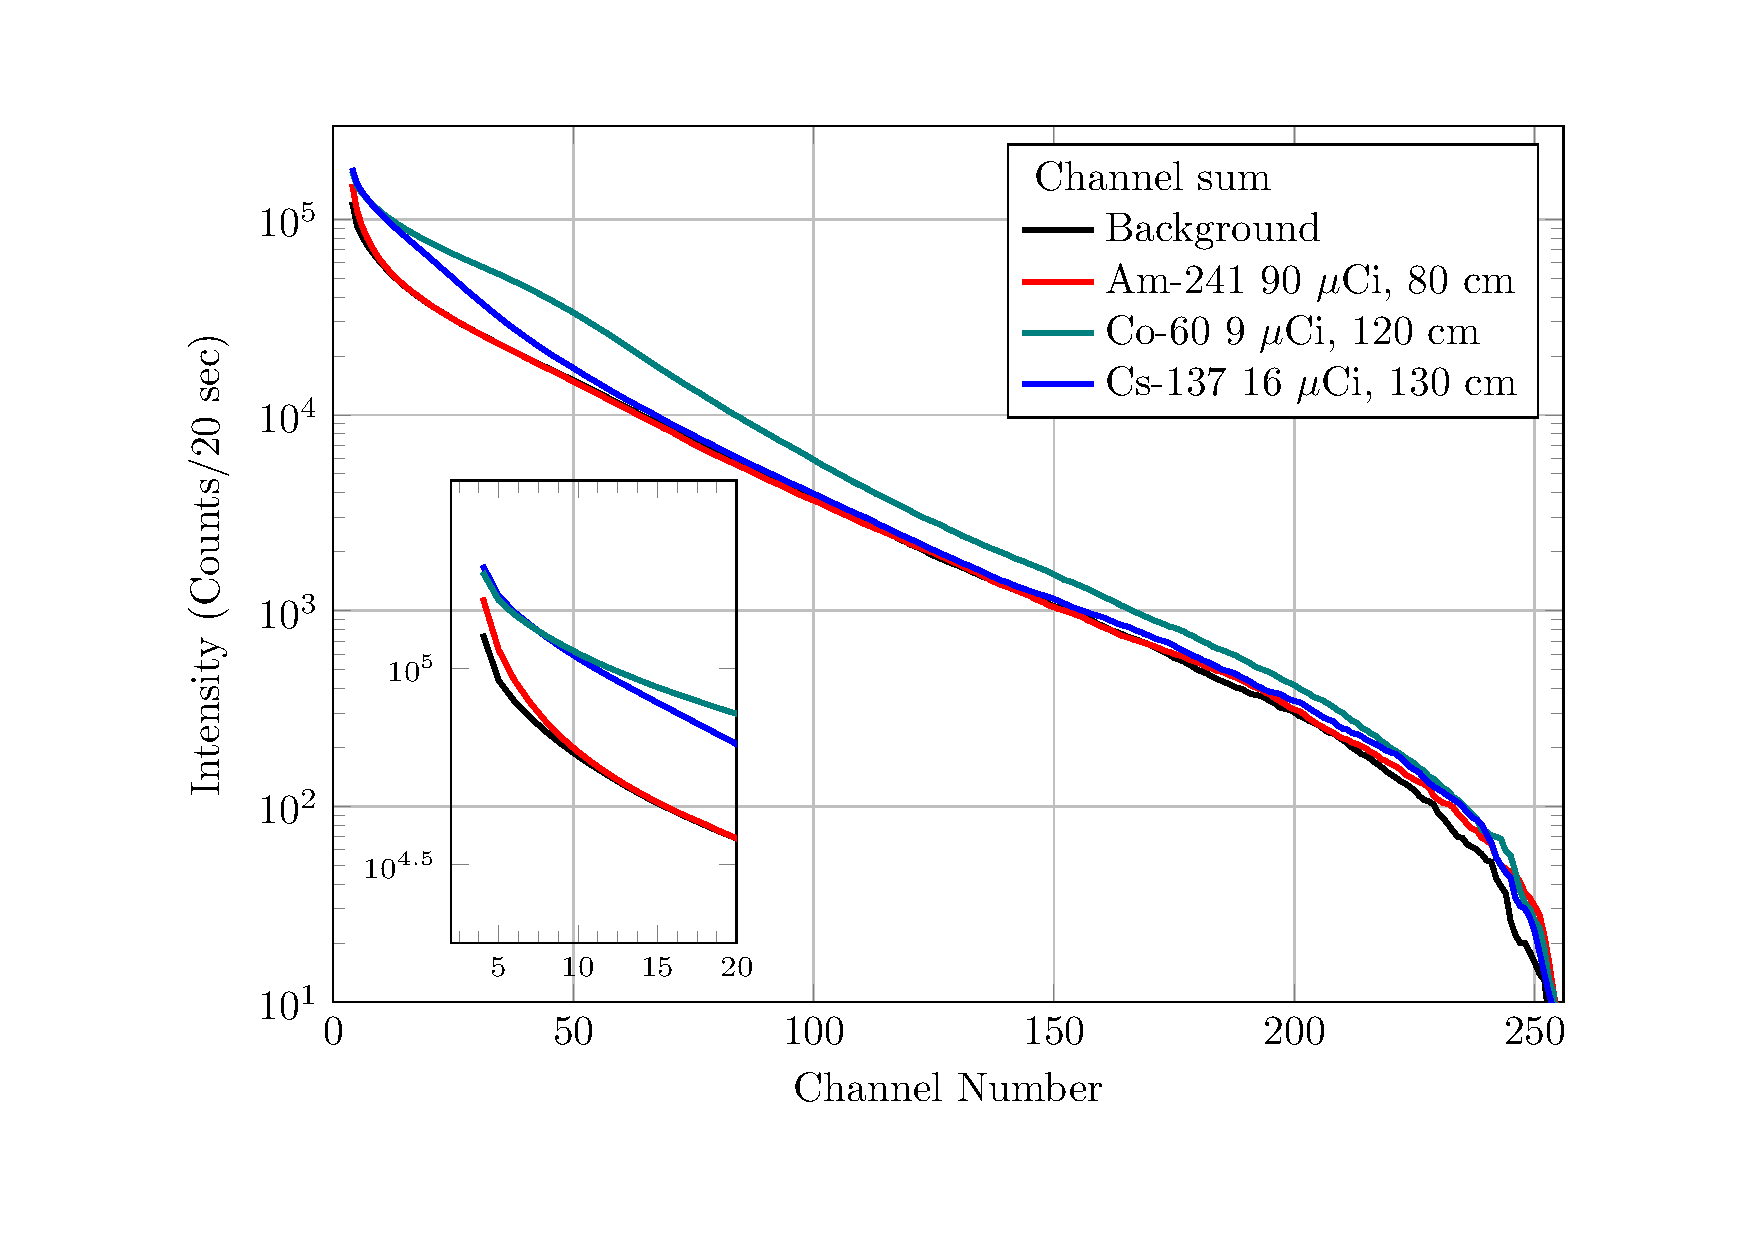
\includegraphics[width=\linewidth]{figure/fig02_channelsum.pdf}
\caption{BCCS-transformed spectra of background (black) and reference radionuclides (Am-241 in red, Co-60 in green and Cs-137 in blue). Backward Cumulative Channel Sum (BCCS) enhances global spectral structure while reducing high-frequency noise. The resulting cumulative spectra show clear separation between radionuclides and background in the low-channel region.}
\label{fig:channelsum}
\end{figure}

\begin{figure}[ht]
\centering
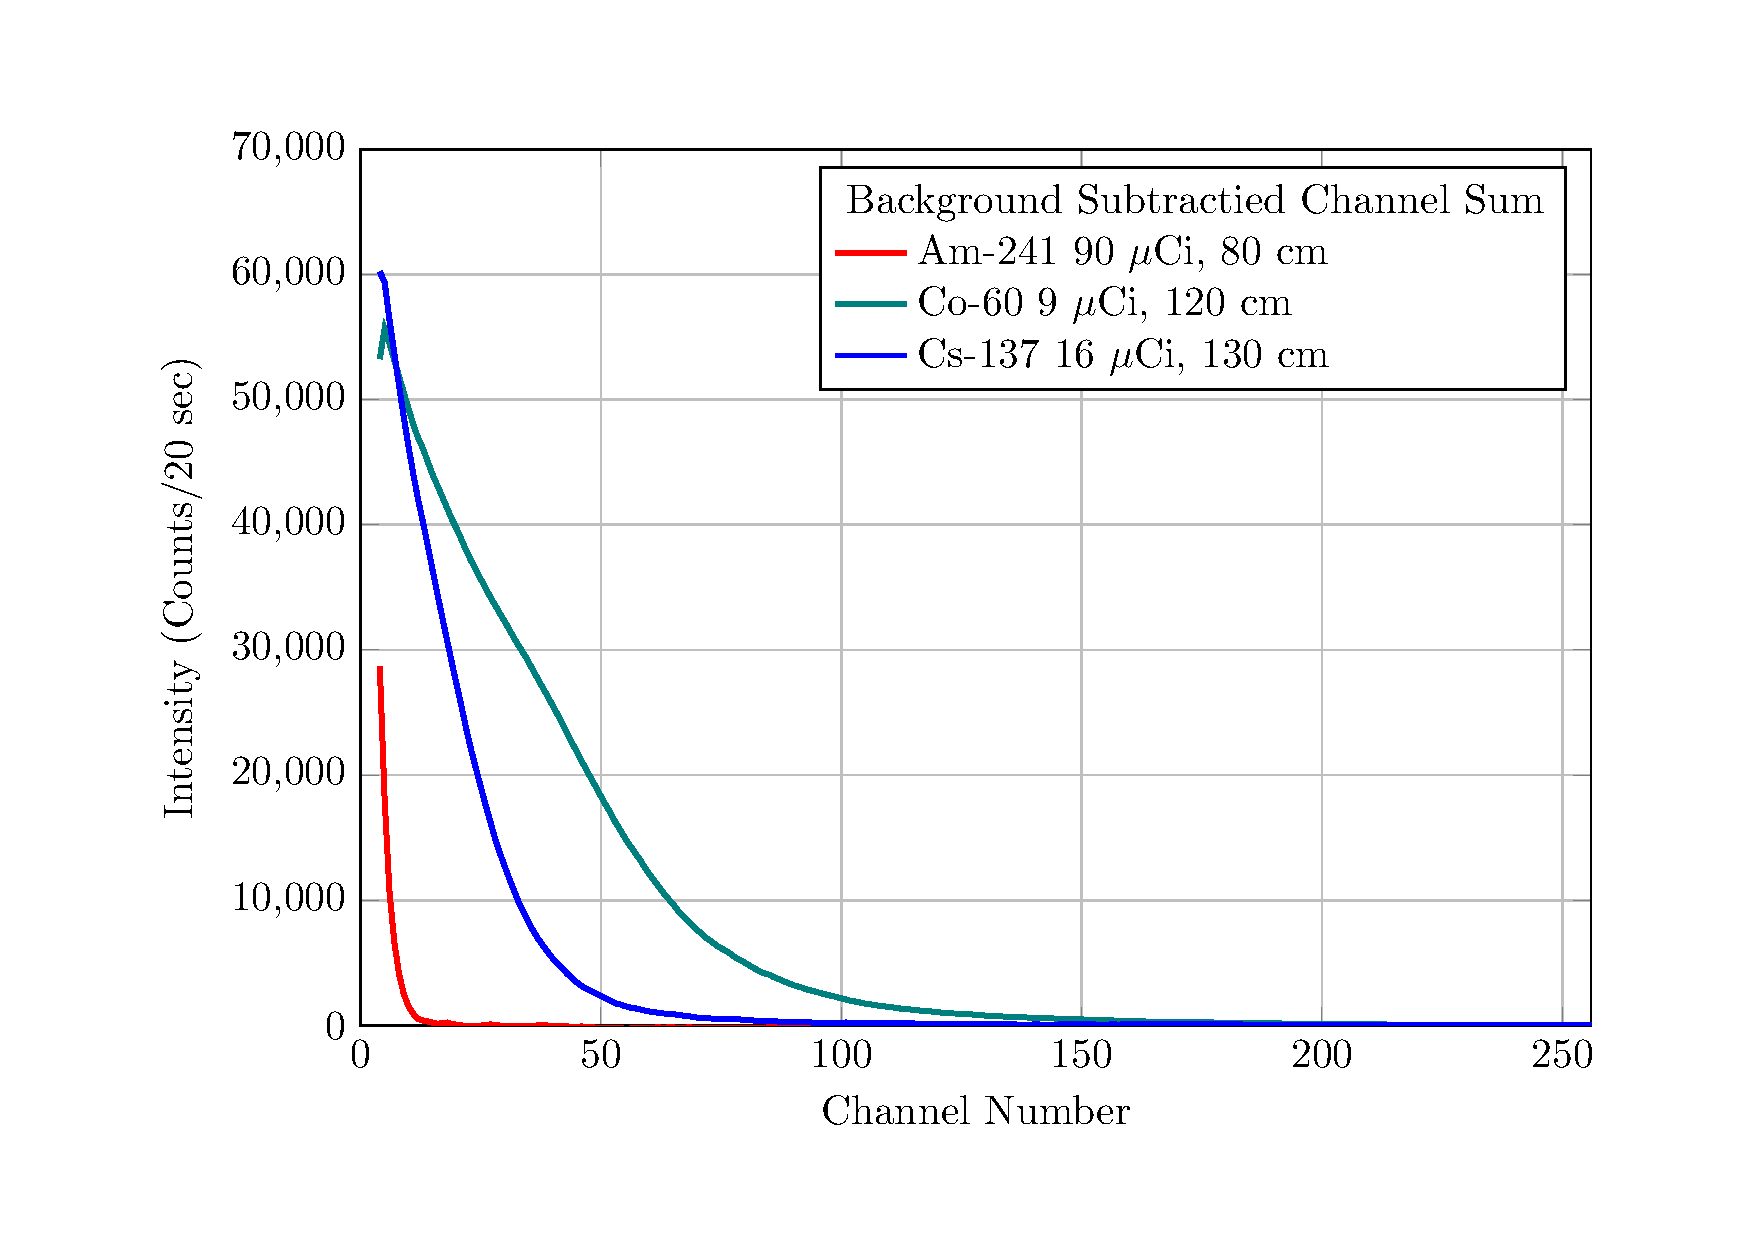
\includegraphics[width=\linewidth]{figure/fig03_csn.pdf}
\caption{Background-subtracted BCCS spectra of Am-241 (red), Cs-137 (green), and Co-60 (blue), obtained by subtracting the background BCCS spectrum (black) from each source spectrum. The subtraction process isolates source-specific spectral features, enhancing separability among the radionuclides.}
\label{fig:csn}
\end{figure}

\begin{figure}[ht]
\centering
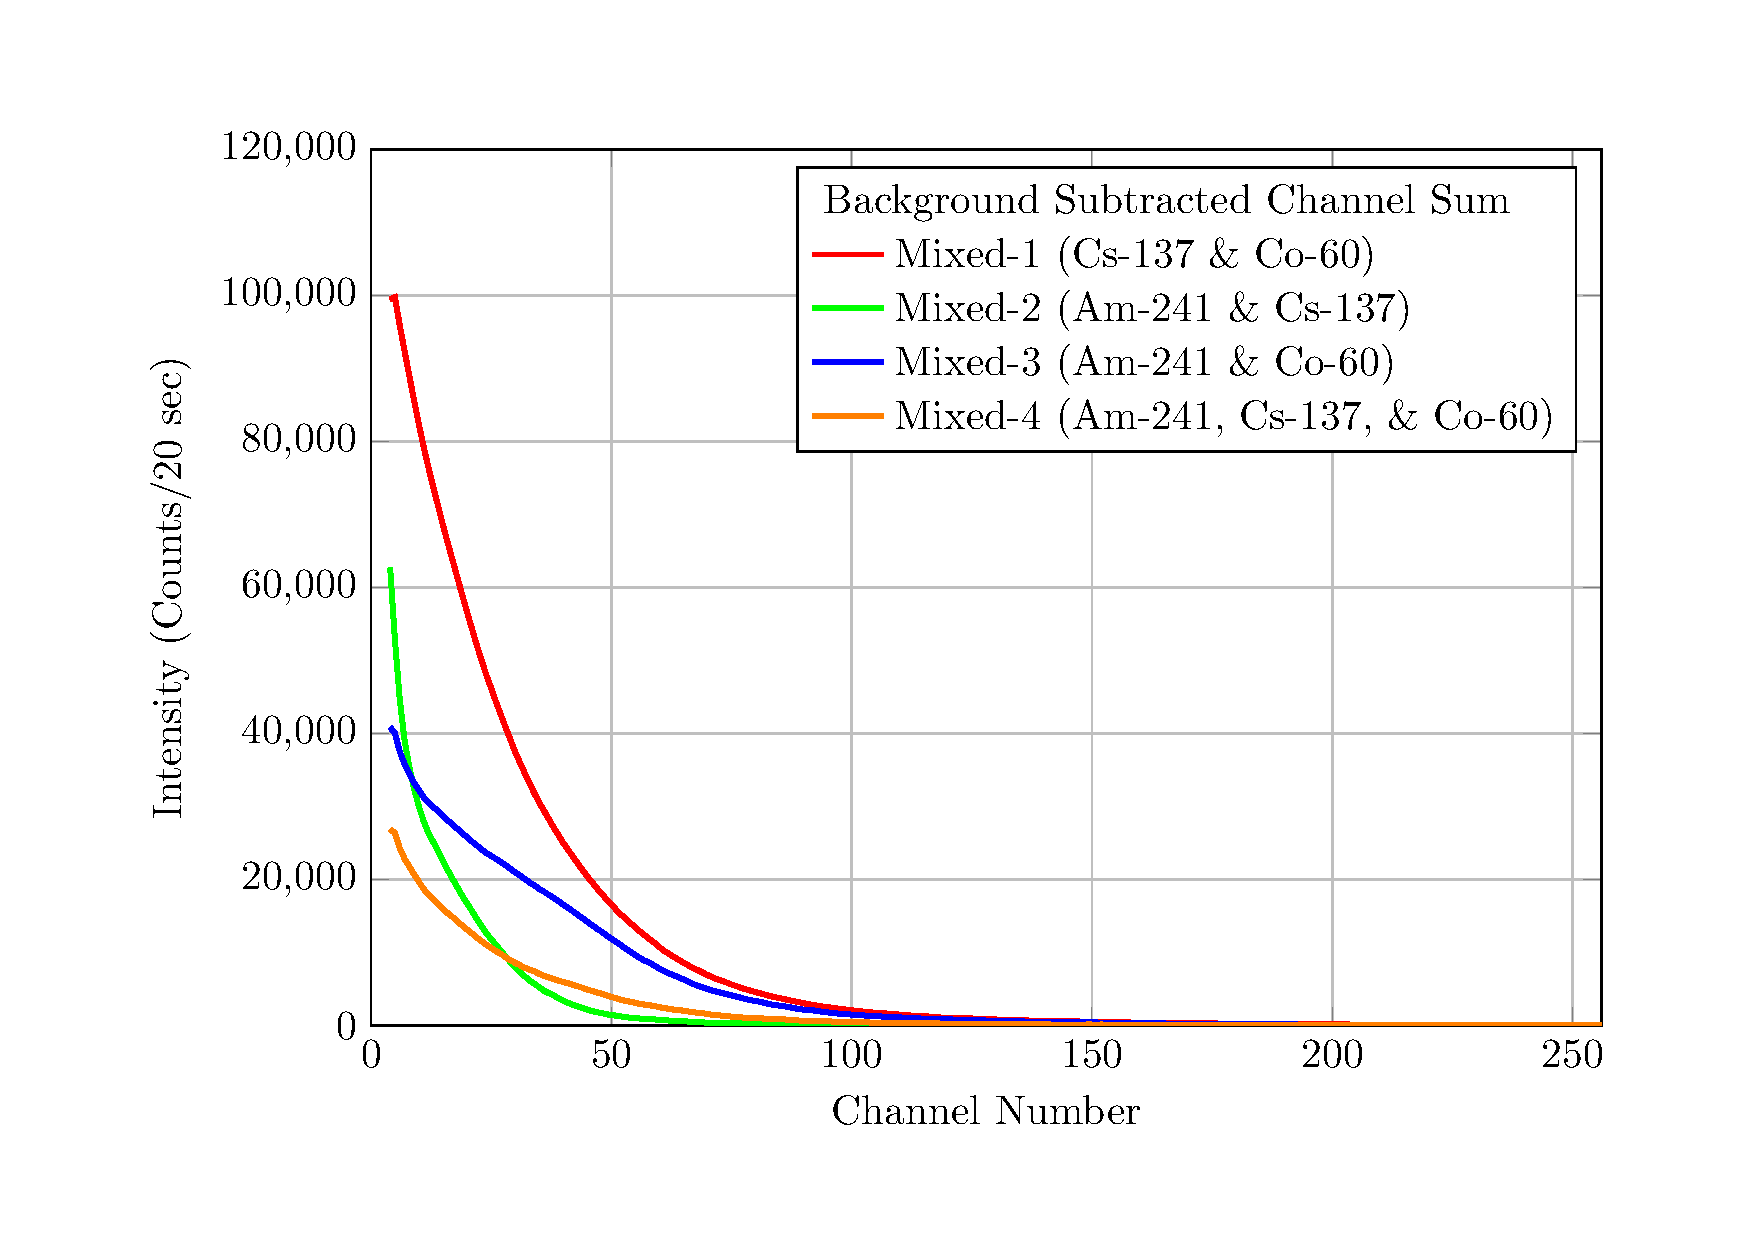
\includegraphics[width=\linewidth]{figure/fig04_CSBS.pdf}
\caption{Background-subtracted  spectra of four mixed radionuclide configurations: Mixed-1 (Cs-137 \& Co-60, red), Mixed-2 (Am-241 \& Cs-137, green), Mixed-3 (Am-241 \& Co-60, blue), and Mixed-4 (Am-241, Cs-137, \& Co-60, cyan). The cumulative profiles retain mixture-specific spectral patterns, supporting quantitative analysis through linear spectral unfolding.}
\label{fig:csbrs}
\end{figure}

\begin{figure}[ht]
\centering
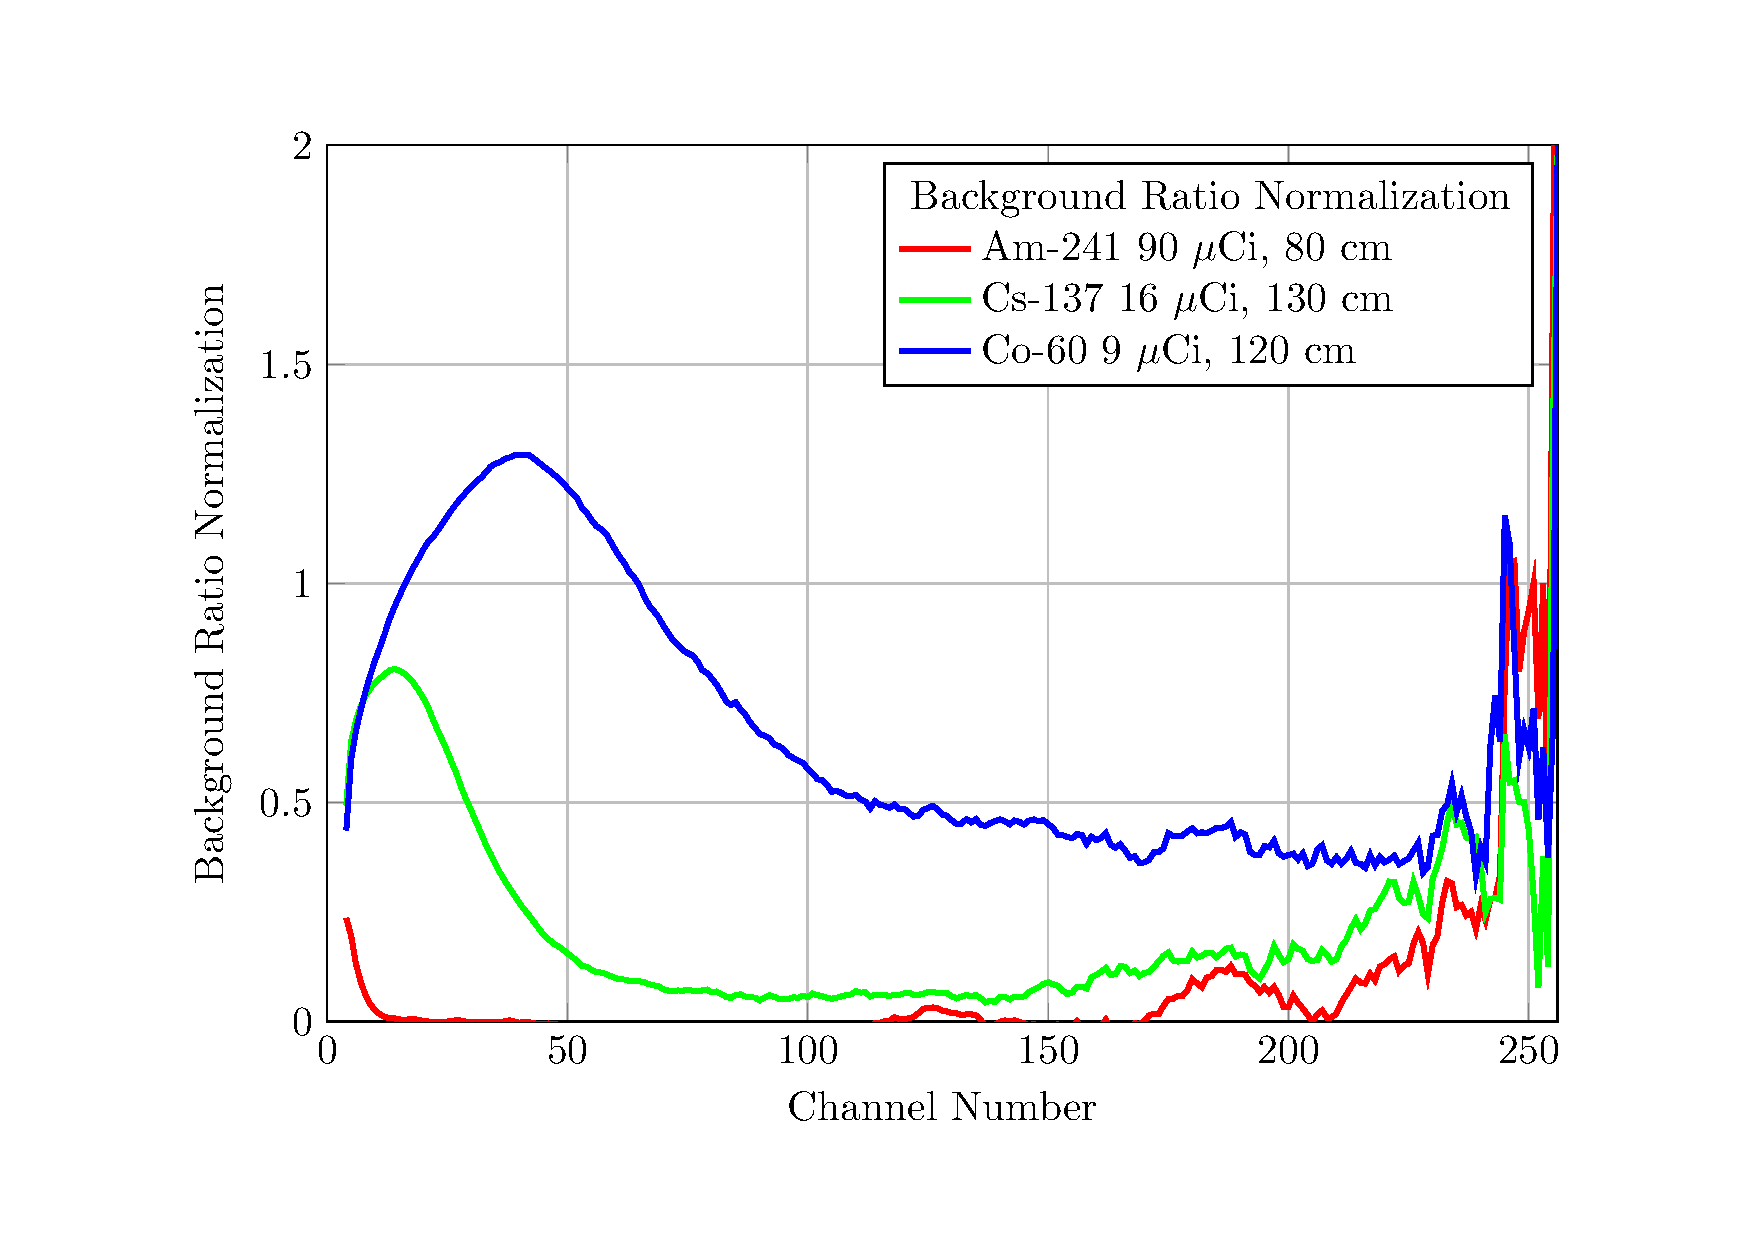
\includegraphics[width=\linewidth]{figure/fig05_CSRN.pdf}
\caption{ Ratio-normalized spectra of single radionuclide—Am-241 (red), Cs-137 (green), and Co-60 (blue)—obtained by computing the channel-wise ratio of the source-plus-background spectrum to the background spectrum. The method emphasizes relative spectral deviations, improving contrast and separability under low-count conditions.}
\label{fig:csbs}
\end{figure}

\begin{figure}[ht]
\centering
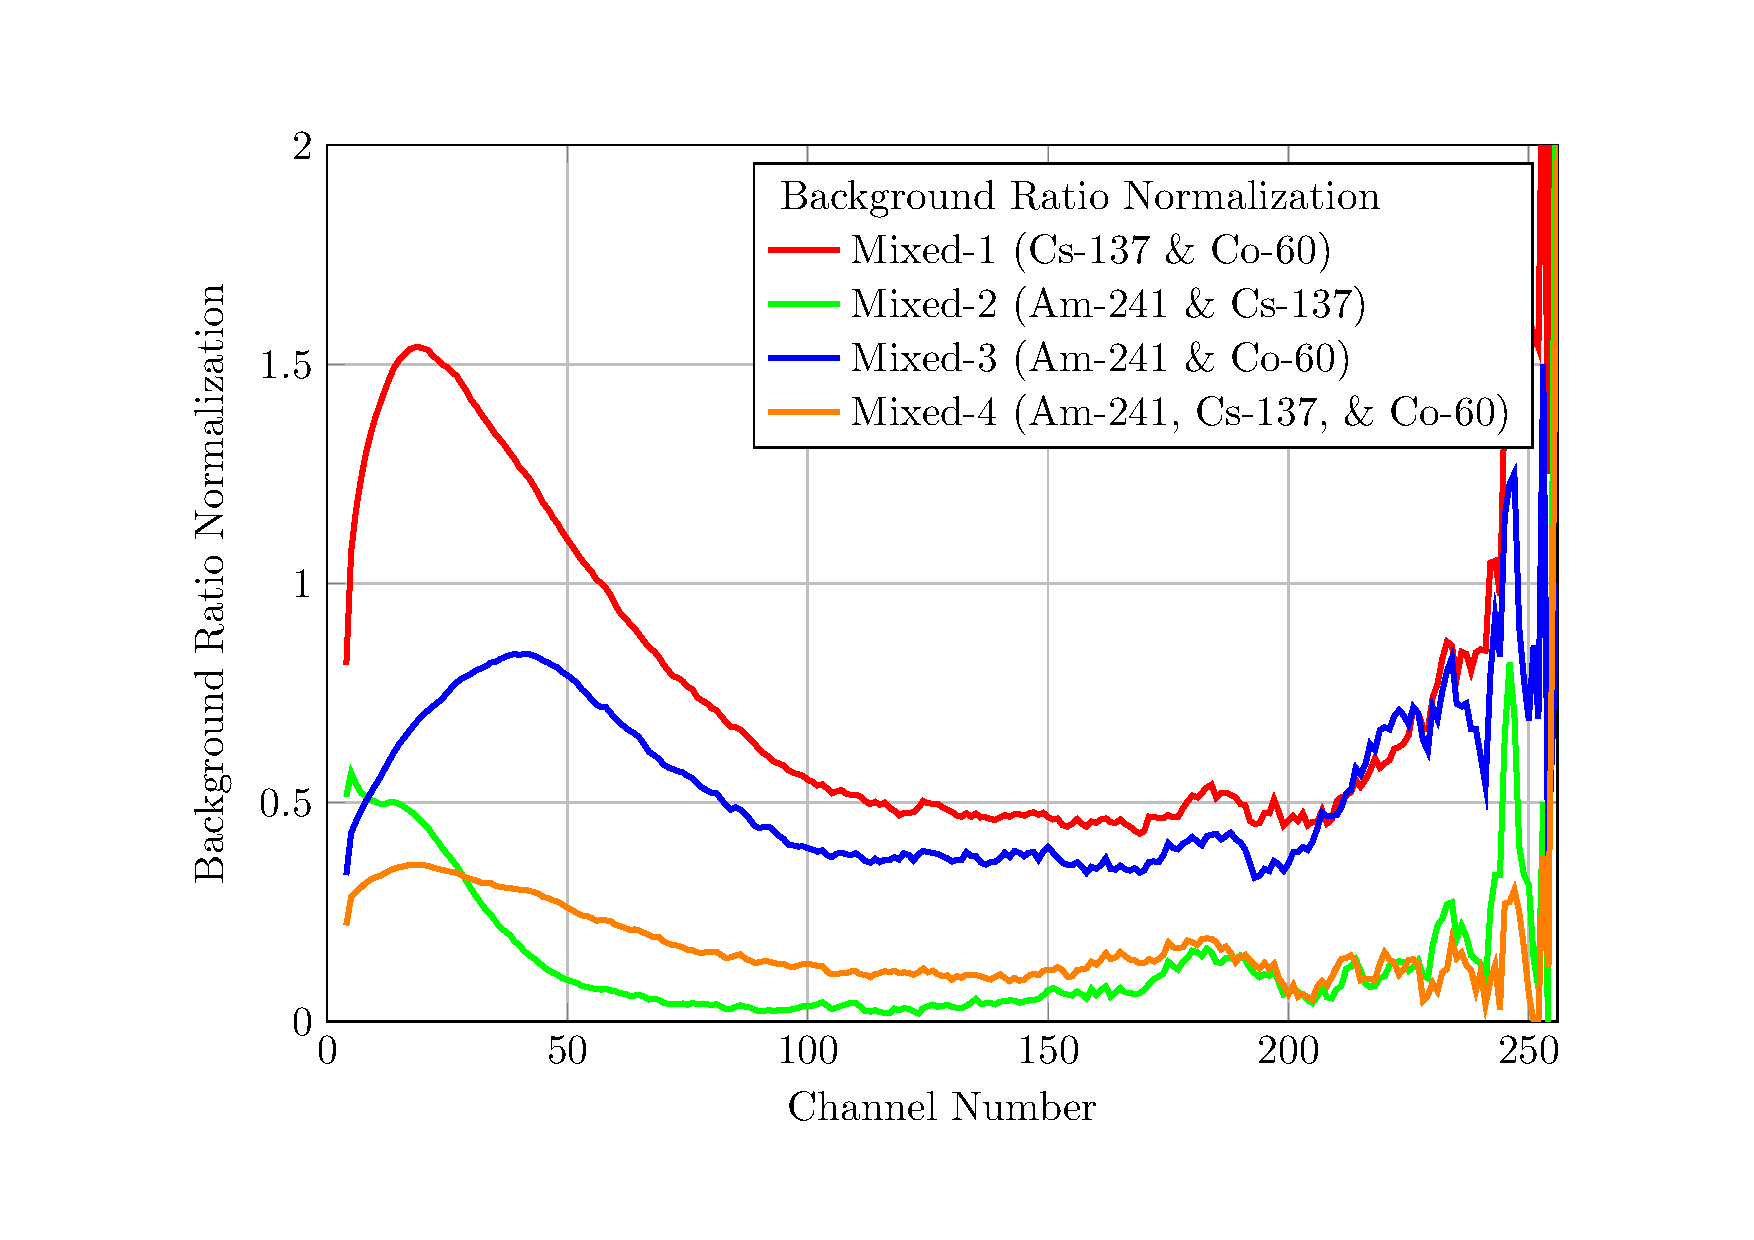
\includegraphics[width=\linewidth]{figure/fig06_CSBRS.pdf}
\caption{Ratio-normalized spectra of four mixed radionuclides configurations: Mixed-1 (Cs-137 \& Co-60, red), Mixed-2 (Am-241 \& Cs-137, green), Mixed-3 (Am-241 \& Co-60, blue), and Mixed-4 (Am-241, Cs-137, \& Co-60, cyan). Ratio-based normalization reveals mixture-specific relative deviations, enabling pattern-based classification and spectral unfolding.}
\label{fig:fi_CSBRS}
\end{figure}

\begin{figure}[ht]
\centering
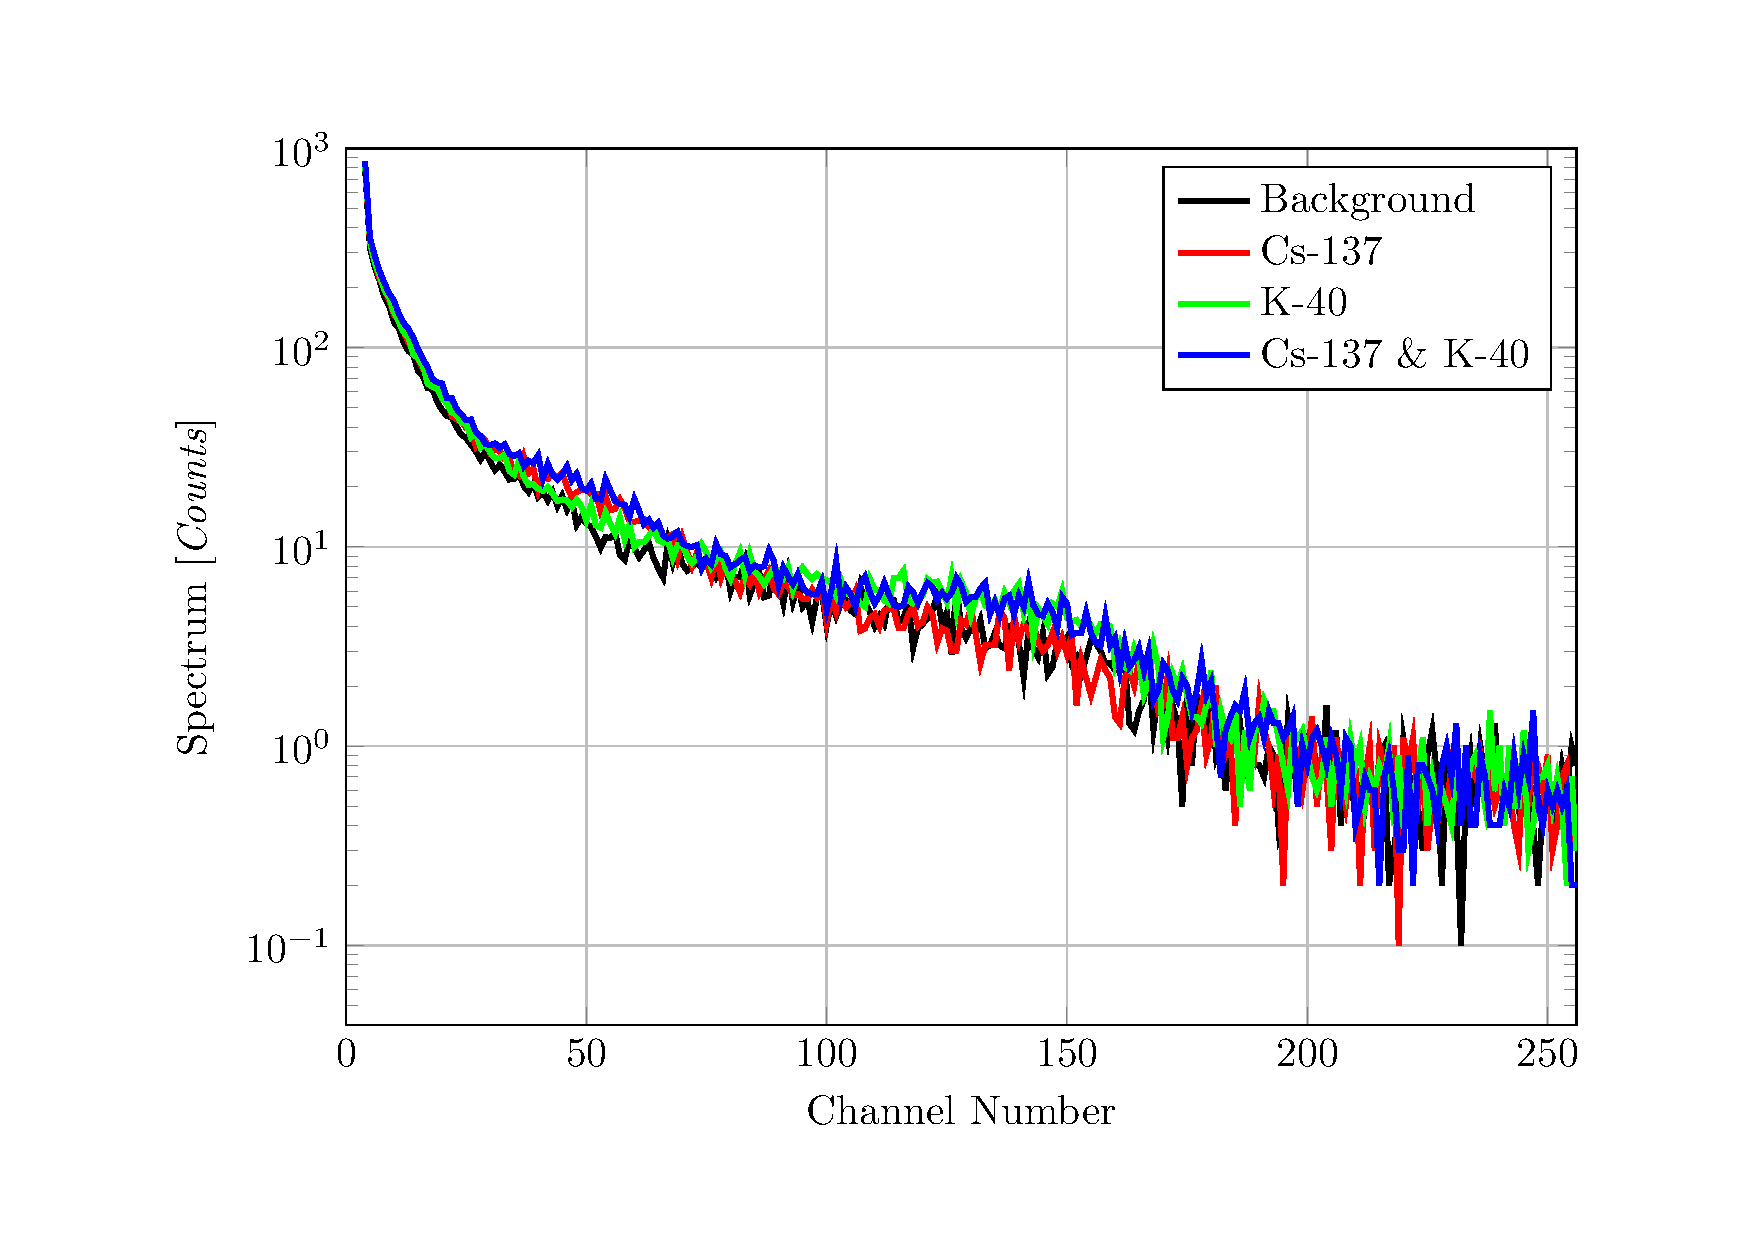
\includegraphics[width=\linewidth]{figure/fig07_FI_SPE.pdf}
\caption{Gamma-ray spectra measured for background (black), Cs-137 (1 kBq, red), K-40 (1 kBq, green), and their combination (blue) using a food radiation screening system. The system successfully distinguishes Cs-137 contamination in food products from the naturally occurring K-40 radiation. Notably, the measured count rates were 428 cps for background, 471 cps for Cs-137, 478 cps for K-40, and 523 cps for the combined sample, representing only about a 10\% increase over background levels. Despite this small difference, repeated measurements showed a statistical uncertainty of less than 5\%, confirming the system's capability to reliably detect such weak contamination signals.}
\label{fig:fi_spe}
\end{figure}

\begin{figure}[ht]
\centering
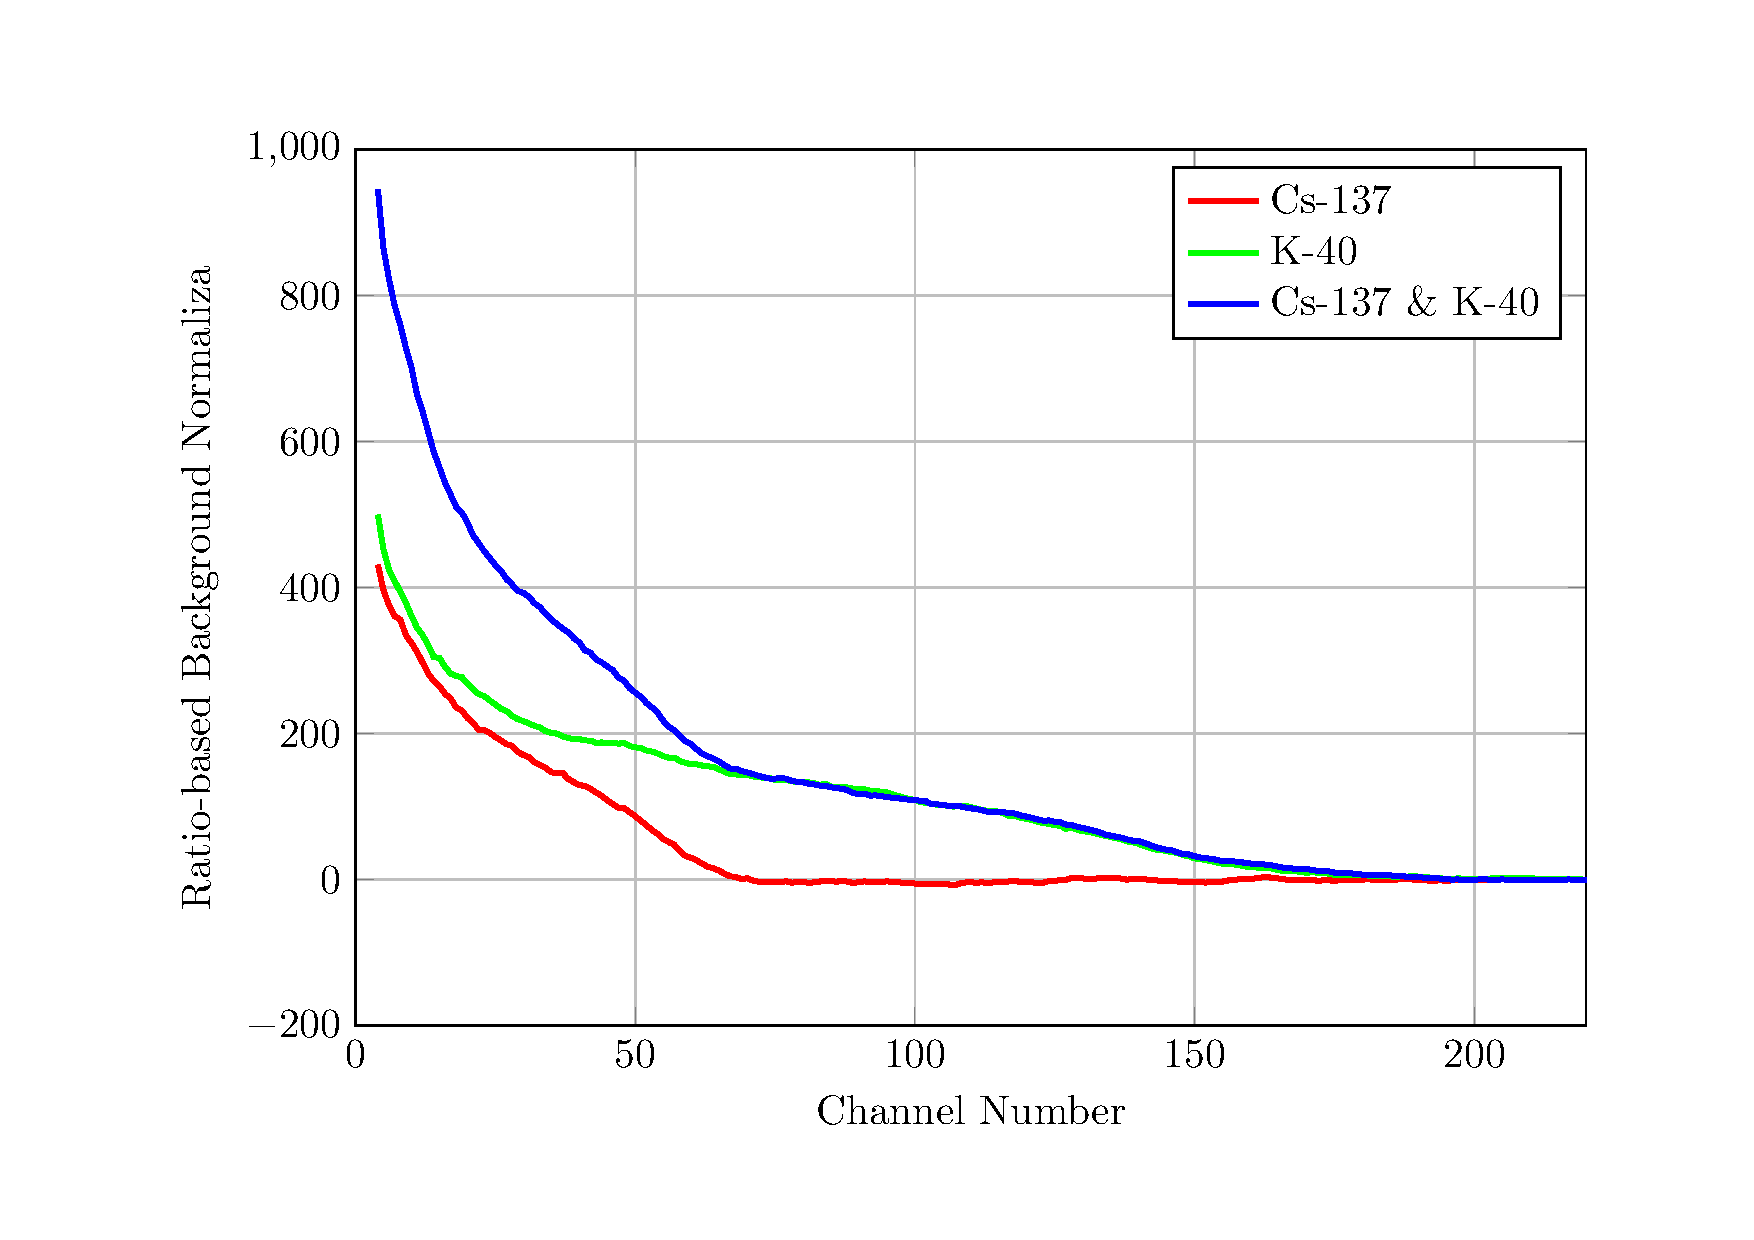
\includegraphics[width=\linewidth]{figure/fig08_FI_CSN.pdf}
\caption{Ratio-based background normalization applied to the measured spectra. This method highlights the spectral differences between Cs-137 and K-40, demonstrating that the food screening system is capable of distinguishing anthropogenic Cs-137 contamination from naturally present K-40 radiation commonly found in foodstuffs such as bananas, seaweed, and salt.}
\label{fig:fi_csn}
\end{figure}

\begin{figure}[ht]
\centering
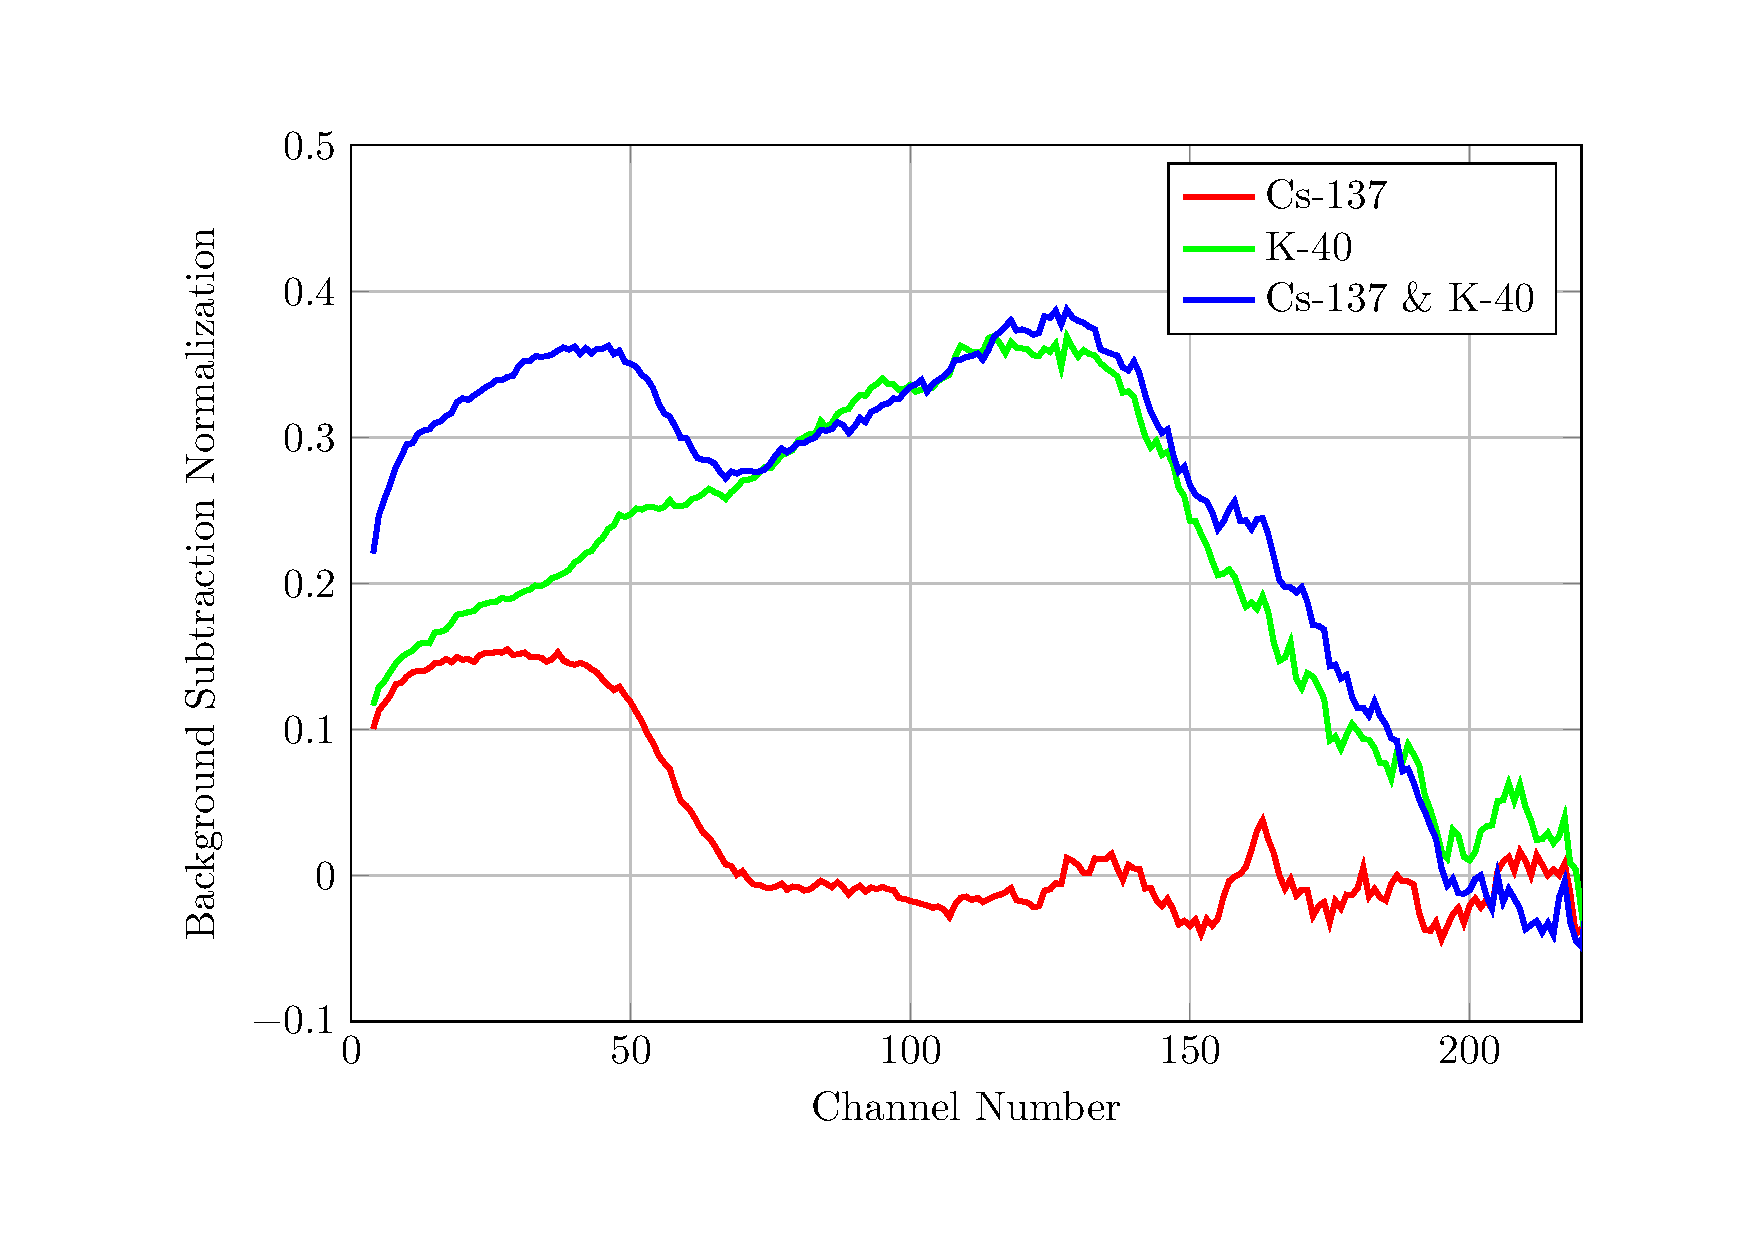
\includegraphics[width=\linewidth]{figure/fig09_FI_CSRN.pdf}
\caption{Background subtraction normalization applied to the measured spectra. After subtracting the background contribution, the net gamma-ray signatures of Cs-137 and K-40 are clearly isolated, showing that the system can differentiate these radionuiclides even under low count conditions. This capability is crucial for food safety monitoring where both artificial and natural radionuclides coexist.}
\label{fig:fi_csbs}
\end{figure}



\begin{figure}[ht]
\centering
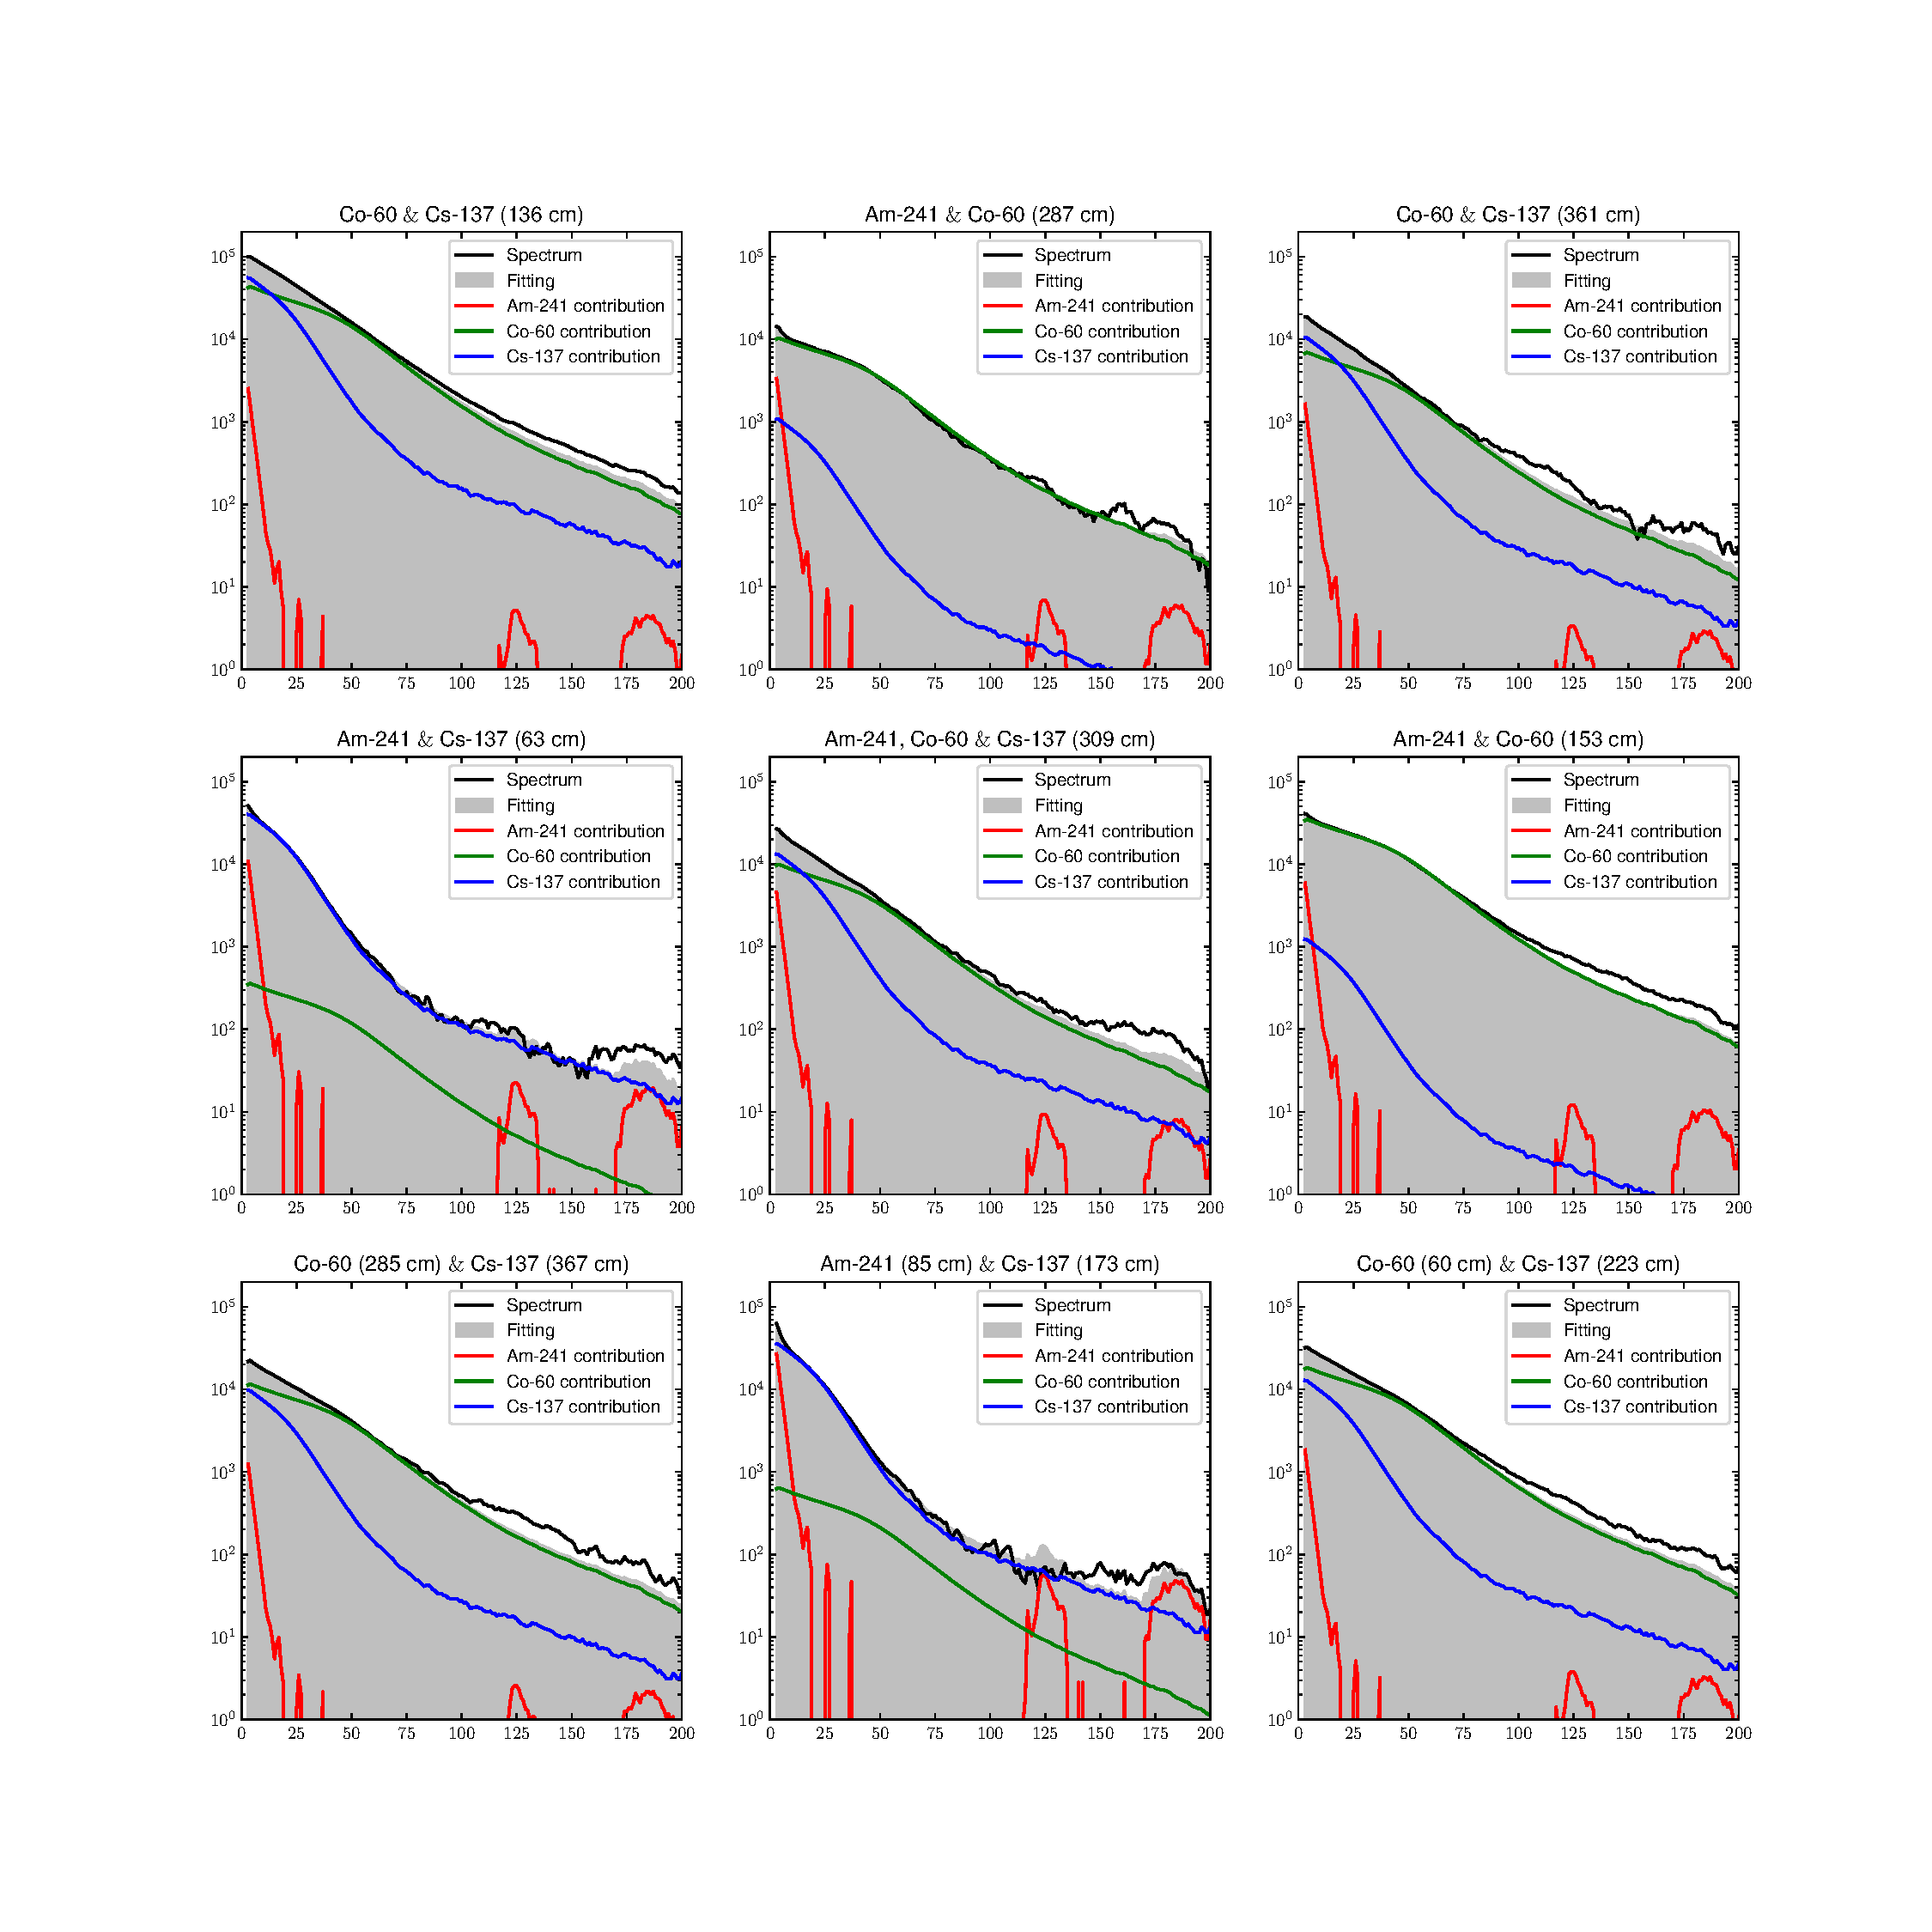
\includegraphics[width=\linewidth]{figure/fit_BGSub.pdf}
\caption{Bacground subtracted fitting result}
\label{fig:fi_fitbgsub}
\end{figure}

\begin{figure}[ht]
\centering
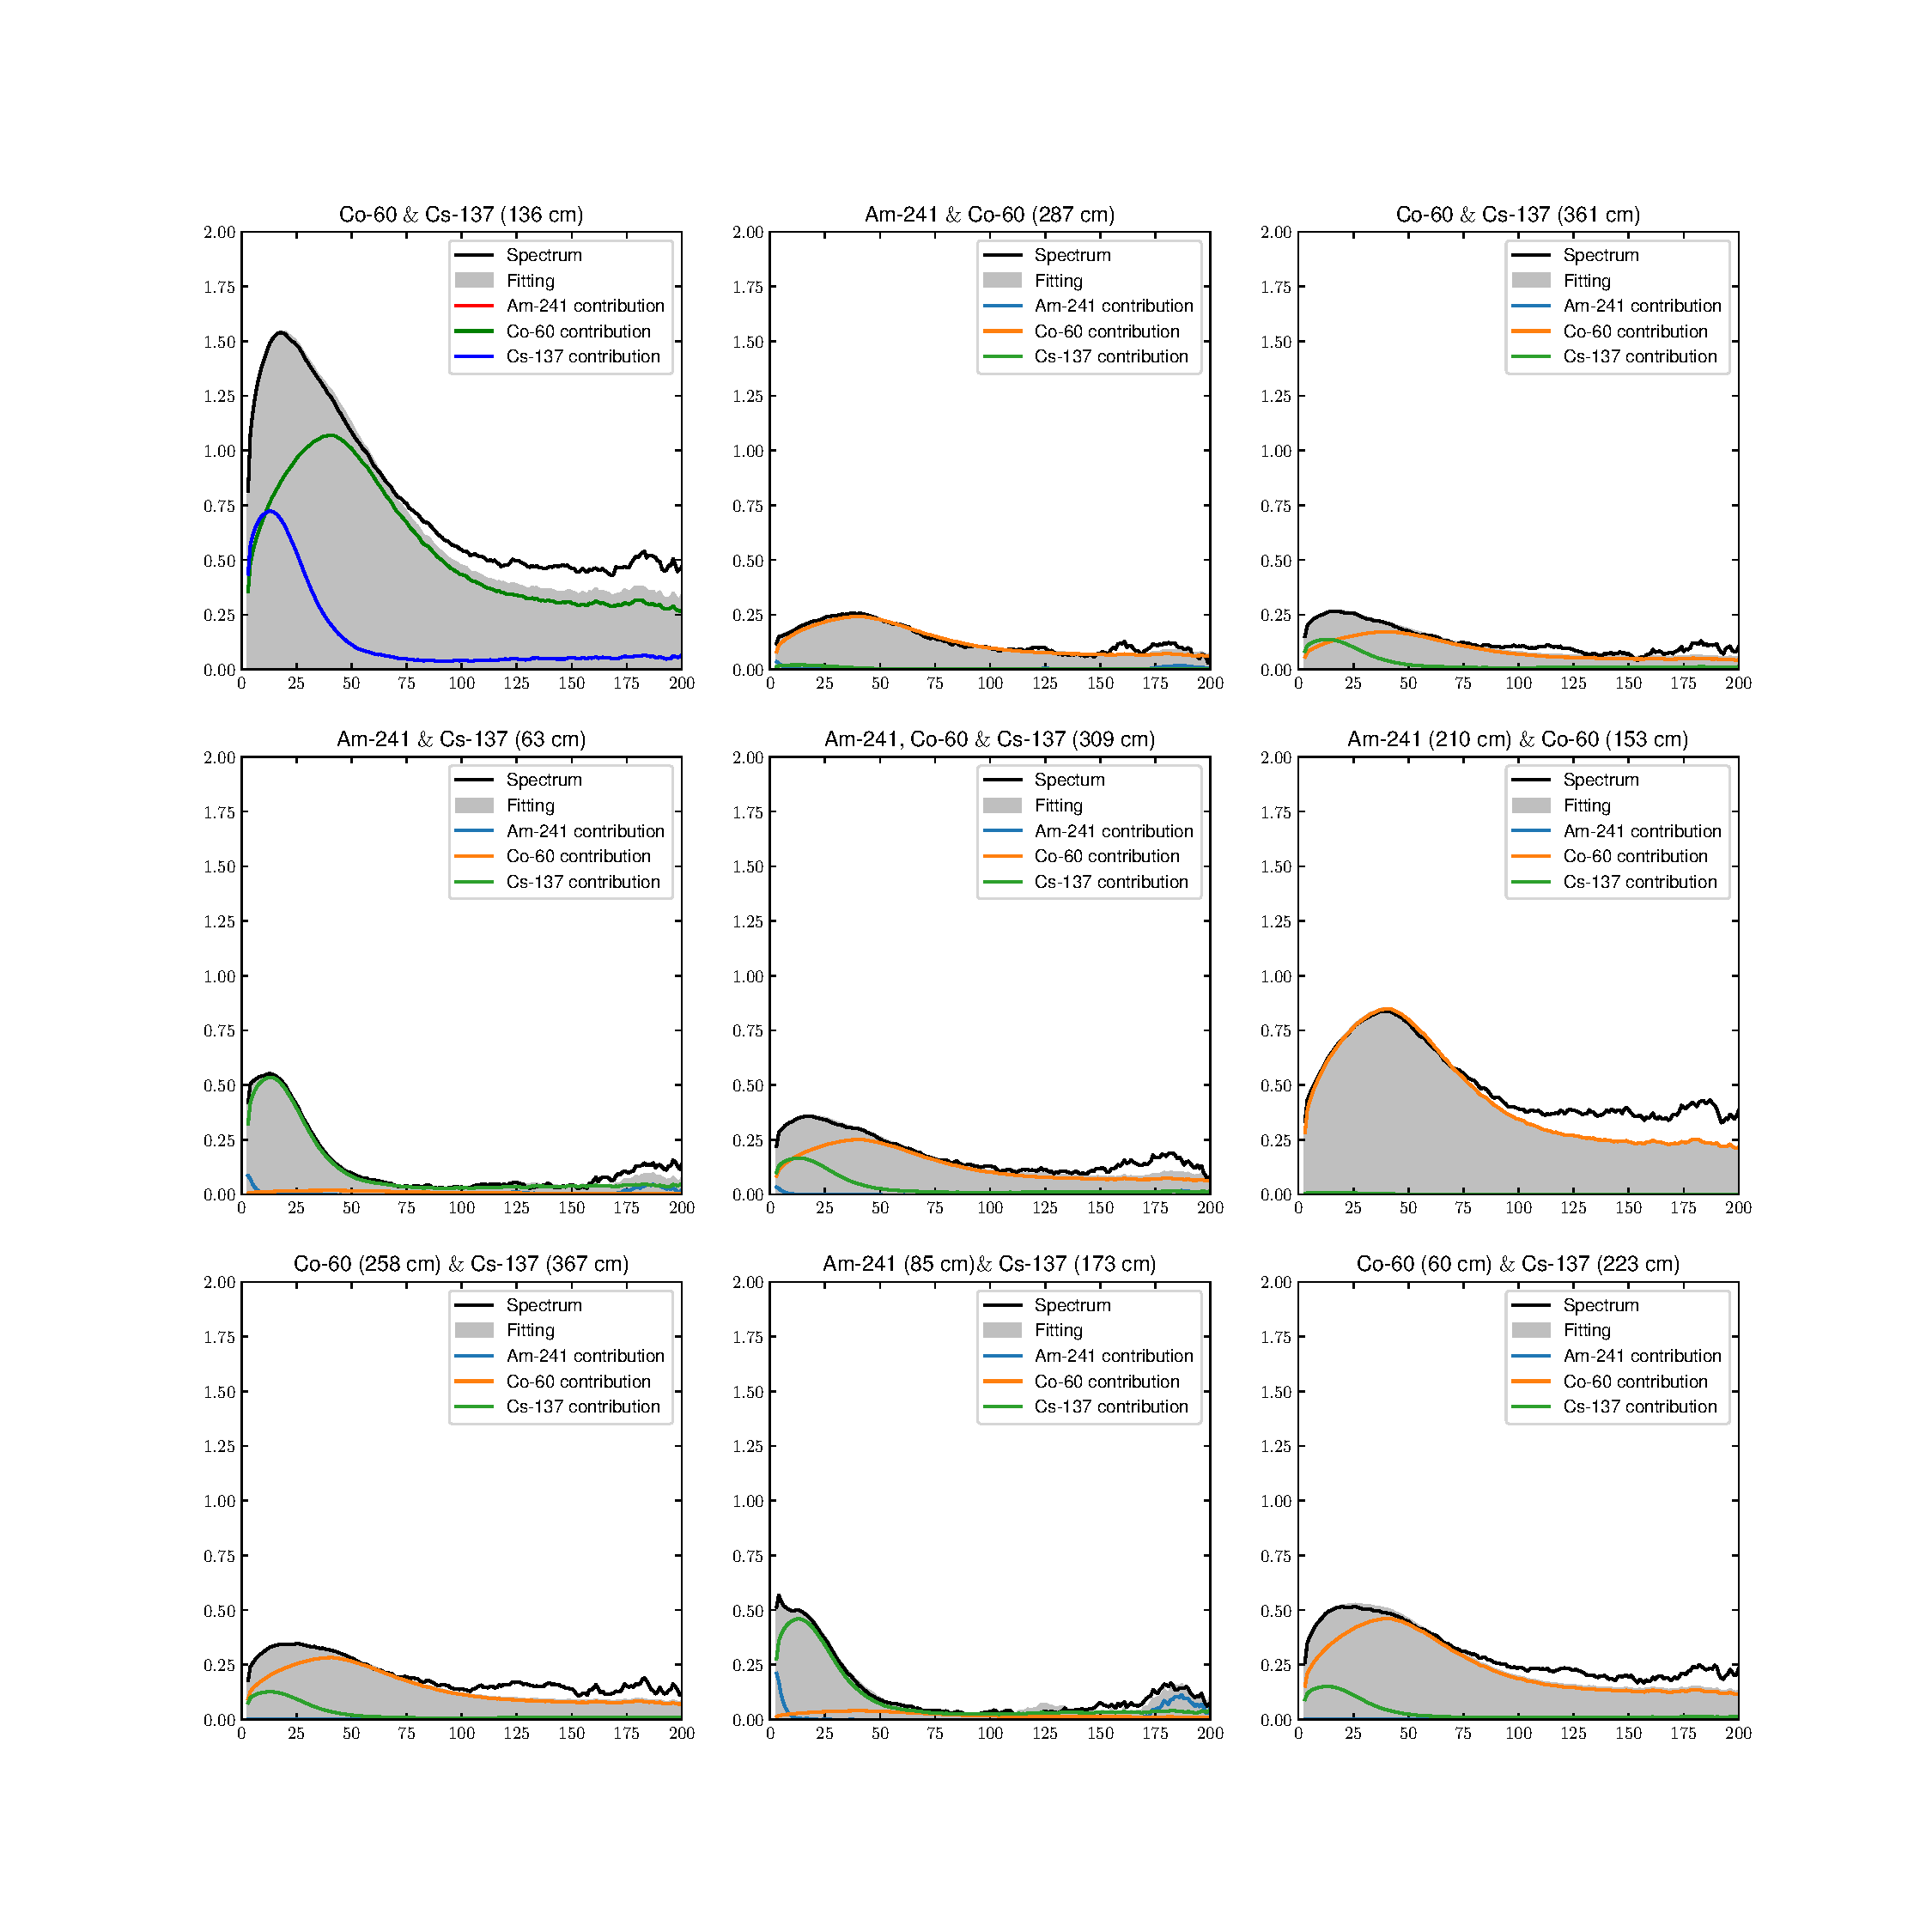
\includegraphics[width=\linewidth]{figure/fit_BGRto.pdf}
\caption{Backgroud ratio fitting result.}
\label{fig:fi_fitbfrto}
\end{figure}

\end{document}